% !TeX root = ../note.tex
\section{Тестирование и отладка}\label{sec:manual}

Тестирование приложения проведено помодульно. Использовался следующий алгоритм тестирования модулей:
\begin{itemize}
    \item реализуется самодостаточная часть нового функционала;
    \item проводится ручное тестирование;
    \item на основе результатов тестирования делается вывод о работоспособности нового модуля;
    \item если в ходе тестирования были выявлены дефекты, то доступная информация о нём записывается и в дальнейшем будет использована для его исправления.
\end{itemize}

\bigskip
\textbf{Тестирование клиентского приложения}

Для валидации и исправления найденных дефектов в клиентском приложении используется инструмент vue-devtools.

vue-devtools – браузерное расширение для отладки приложений Vue.js, однако его можно использовать только во время разработки. Он содержит в себе следующий функционал:
\begin{itemize}
    \item обзор всех компонентов и их содержимого на текущей странице;
    \item текущий навигационный маршрут и историю их изменений;
    \item вызываемые компонентами события и параметры, передающиеся ими.
\end{itemize}

Благодаря полученной с помощью инструмента информации, разработчик может максимально эффективно обнаруживать ошибки и исправлять их в клиентской части ПС. На рисунке~\ref{fig:vue_js_devtools} приведён пример интерфейса vue-devtools.

\begin{figure}[h]
    \centering
    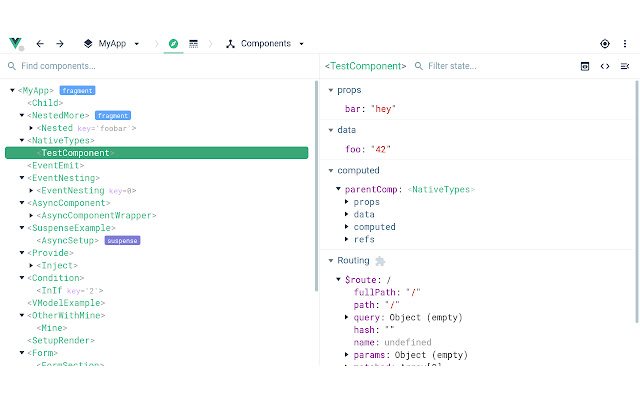
\includegraphics[width=\textwidth]{vue_js_devtools}
    \caption{Пример интерфейса vue-devtools}\label{fig:vue_js_devtools}
\end{figure}

\bigskip
\textbf{Тестирование .NET сервисов}

Для работы с дефектами в .NET сервисах используются следующие инструменты:
\begin{itemize}
    \item отладчик Visual Studio;
    \item логирование ошибок.
\end{itemize}

Отладчик — это узкоспециализированное средство разработки, которое присоединяется к работающему приложению и позволяет проверять код. В отладчике доступно множество способов наблюдения за выполнением кода. Есть возможность пошагово перемещаться по коду и просматривать значения, хранящиеся в переменных, задавать контрольные значения для переменных, чтобы отслеживать изменение значений, изучать путь выполнения кода и т. д.

Пошаговое исполнение кода может занять продолжительное время, поэтому в проекте также используется логирование, которое значительно сокращает время отладки ошибки. Также логирование позволяет получать информацию о состоянии программного средства даже на тех машинах, к которым у нет физического доступа. 

Таким образом, было проведено ручное тестирование всех сервисов. Были использованы наиболее эффективные инструменты тестирования и отладки, что позволяет заявить о высоком качестве и надёжности программного средства.
